\section{Durchführung}
\label{sec:Durchführung}

\begin{figure}[H]
    \centering
    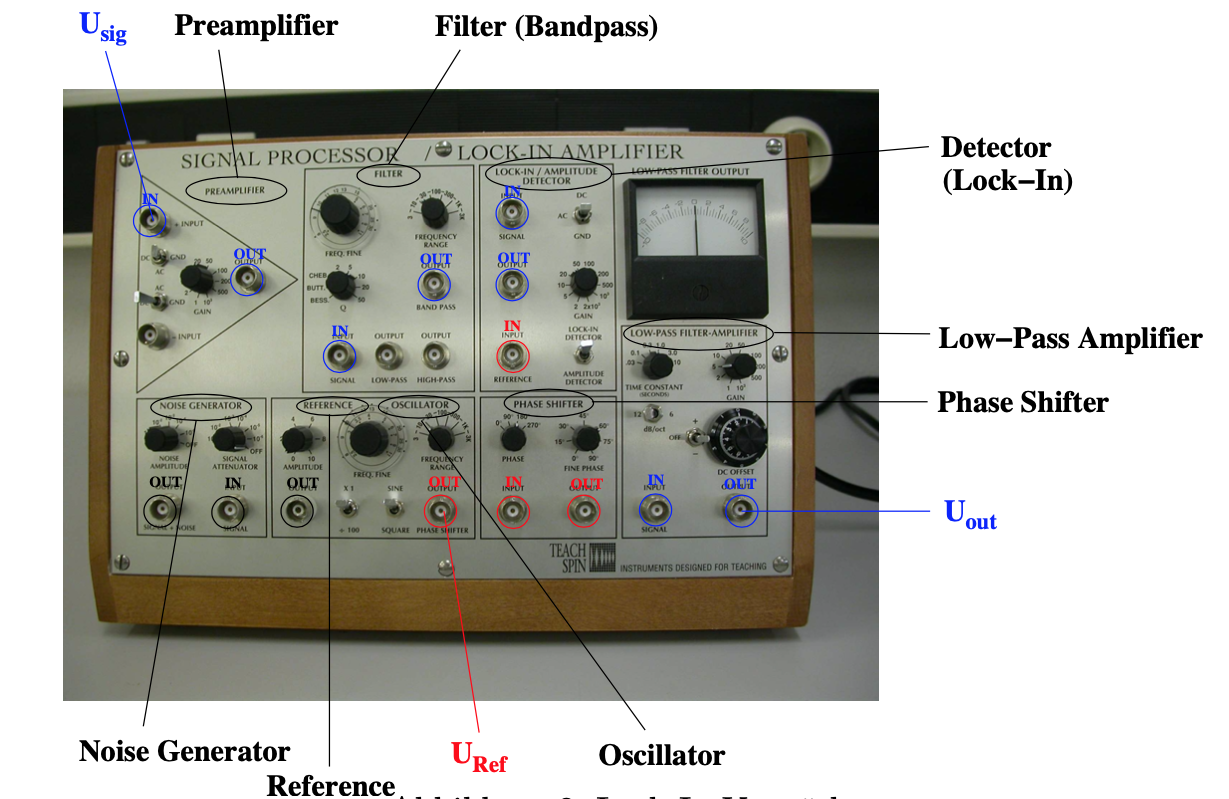
\includegraphics[scale=1]{content/lock_in_gerät.png}
    \caption{Der in diesem Versuch genutzte Lock-In-Verstärker. Quelle:\cite{sample}}
    \label{fig:Prinzip_lock_in}
\end{figure}


Im ersten Teil soll die Funktionsweise des Lock-In-Verstärkers untersucht werden.\\

Es wird dazu die folgende Schaltung verwendet.

\begin{figure}[H]
    \centering
    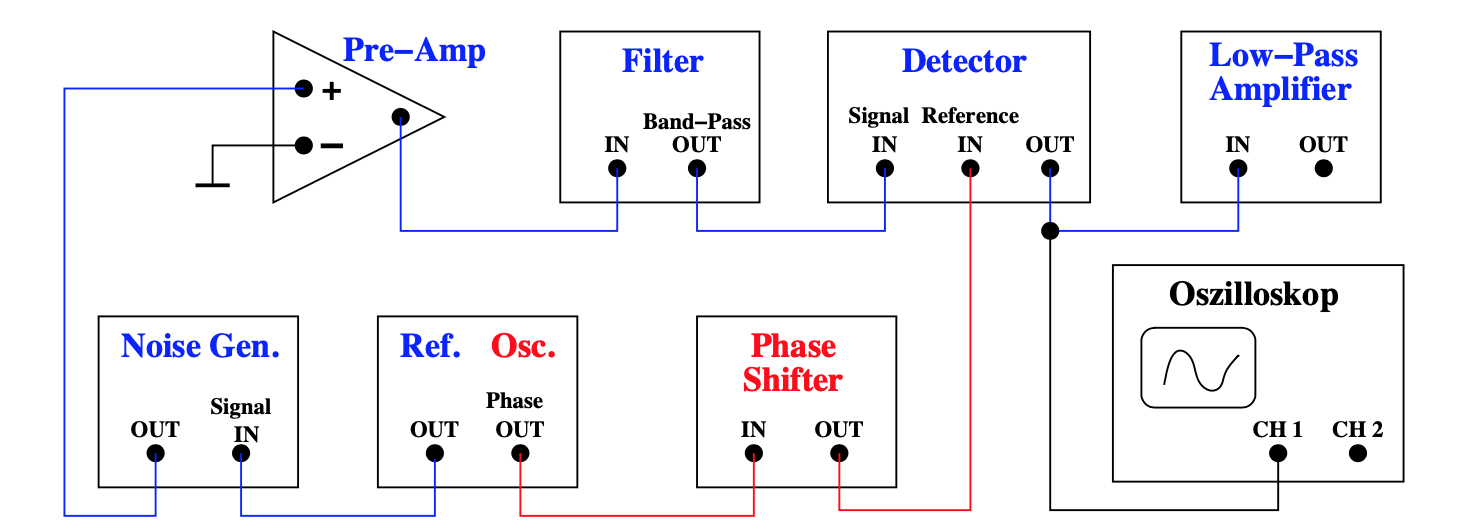
\includegraphics[scale=1]{content/esb_teil1.png}
    \caption{Das ESB des ersten Versuchsteils. Quelle:\cite{sample}}
    \label{fig:Prinzip_lock_in}
\end{figure}

Die Phase $\phi$ wird am Phasenschieber in 30°-Schritten hochgestellt und bei jedem Schritte
die Amplitude des Ausgangssignals dokumentiert.\\

Im ersten Messdurchgang wird der Noise Generator abgeschaltet bzw. überbrückt, im Zweiten nicht.

Der zweite Teil des Versuchs besteht darin, den maximalen Abstand
einer LED von einer Photodiode zu ermitteln, bei dem die Photodiode getriggert wird.\\
Die folgende Schaltung wird verwendet.

\begin{figure}[H]
    \centering
    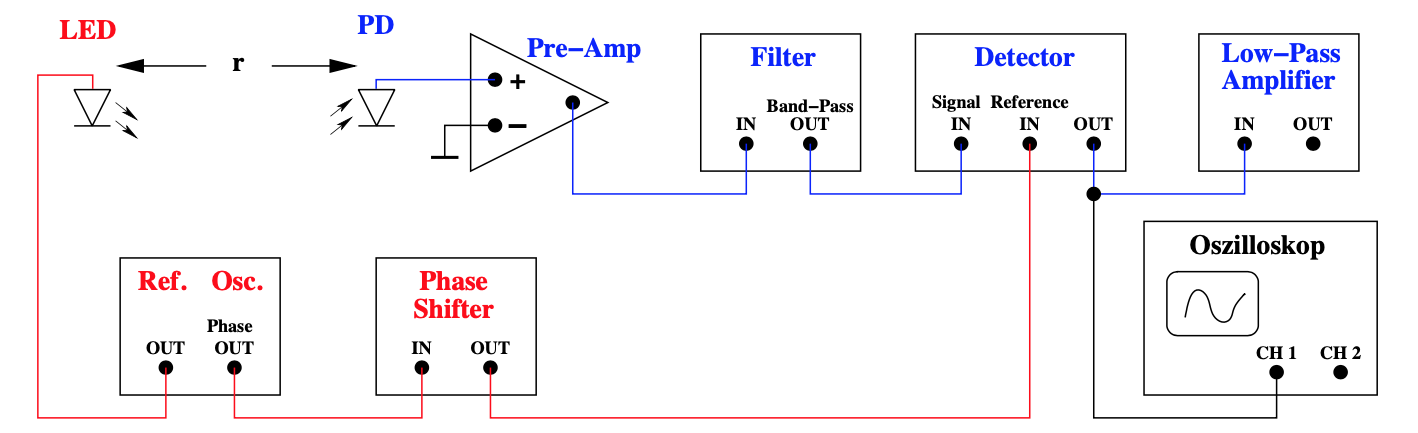
\includegraphics[scale=1]{content/esb_teil2.png}
    \caption{Das ESB der Messung des maximalen Abstands zwischen LED und Photodiode. Quelle:\cite{sample}}
    \label{fig:Prinzip_lock_in}
\end{figure}

